\documentclass{article}
\usepackage{amsmath,amsthm,amssymb}
\usepackage{mathtext}
%\usepackage[T2A]{fontenc}
%\usepackage[utf8]{inputenc}
\usepackage[english]{babel}
\usepackage{graphicx}
\usepackage{hyperref}


\title{Sentiment classification using transformers and capsules: GermEval 2017}
\author{Alexander Pimenov}
\date{May 2020}



\begin{document}
\maketitle
\begin{abstract}
    We perform comparison of performance of several transformer based architectures on GermEval 2017 sentiment classification task. We demonstrate the effectiveness of transfer learning using pretrained BERT and GPT-2 as backbone networks applied with usual classification heads and heads containing capsule layers with Heinsen routing, which after fine tuning can produce state of the art (SOTA) results on the considered dataset.
\end{abstract}



\section{Introduction}

GermEval 2017 competition presented an important challenge to the community in application of state of the art approaches to the automatic extraction of useful information from the texts expressing public opinions about the quality of service of German railway service Deutsche Bahn (DB), which can help them to improve the quality of their services \cite{germevaltask2017}. With the appearance of different attention-based transformer architectures in the last two years the capacity of learning from real text data greatly increased, which is now a subject of extensive research, however this particular dataset was not in particular focus, and this study aims at bringing some understanding on the applicability of transformers to German opinion dataset.  On the other hand, the capsule neural networks (CapsNets) were advertised recently as an approach alternative to convolutional neural networks (CNNs) which aims at eliminating some of the drawbacks of CNNs such as inefficient learning of spatial relations between various features. This problem is very important in NLP as well and is one of the reasons why CNNs had only limited success in applied problems. There are only several works at the moment devoted to the application of CapsNets in NLP with various static and dynamic routing schemes \cite{kim2020text}, which demonstrate their potential, and they were typically successfully applied in combination with other proven mechanisms such as attention layers \cite{xiao2018mcapsnet} and recurrent neural networks \cite{wang2018attention}. In particular, it was suggested basing on one study that one can use pretrained embeddings from the hidden layers of GPT-2 network \cite{radford2019language} as an input to CapsNet to demonstrate state of the art results on the Stanford Sentiment Treebank dataset \cite{heinsen2019algorithm}. In the current work, we extend this idea by applying this architecture to GermEval 2017 sentiment classification task, exploring BERT backbone \cite{devlin2018bert}, and training CapsNet and transformer networks together to obtain SOTA results\footnote{The code is available at https://github.com/DrFirestream/NLP}. 


%\subsection{Team}
%Please list your team members and describe their responsibilities. Example:

%\textbf{Valentin Malykh} prepared this document.



\section{Related Work}
\label{sec:related}

All participants of GermEval 2017 attempted sentiment classification task, and two works were performed after the contest, which demonstrated improvements over the F1 micro average score of the participating solutions \cite{germevaltask2017, biesialska2020sentiment}. Moreover, there is a recent blog post \cite{kostic2020}, which fine-tunes pretrained German BERT network with plain classification head and reports the results that can be considered as the current SOTA on GermEval 2017 test datasets in few epochs. Other approaches use various preprocessing techniques, employ SentiWS lexicon \cite{schulz2017germeval, hovelmann2017fasttext, sidarenka2017potts}, construct SentiWordNet lexicon using the Open Subtitle Corpus \cite{naderalvojoud2017germeval}, obtain embeddings using Sent2Vec and SIF with Word2Vec \cite{lee2017ukp}, TF-IDF and Word2Vec\cite{ruppert2017lt}, GloVe \cite{mishra2017, biesialska2020sentiment} and ELMo \cite{biesialska2020sentiment}. In order to perform sentiment classification, some consider approaches without neural networks such as threshold based classification \cite{schulz2017germeval} and SVMs \cite{sidarenka2017potts}, however most authors employ neural networks such as bidirectional LSTM \cite{sidarenka2017potts, mishra2017, naderalvojoud2017germeval, lee2017ukp} and attention model with transformer encoders \cite{biesialska2020sentiment}. Ensemble approaches combining SVM with LSTM \cite{sidarenka2017potts}, using FastText  \cite{hovelmann2017fasttext} and gradient boosting trees \cite{hovelmann2017fasttext, sayyed2017idst} were also employed.

\section{Model Description}
We consider a model with standard backbones BERT/GPT-2, where the output of the hidden encoder/decoder layers is fed into the CapsNet depicted on \ref{fig:arch}. For comparison, we replace steps (b)-(e) with simple classification head involving batch normalization layer and a fully connected layer. 
 

\begin{figure}[!tbh]
    \centering
    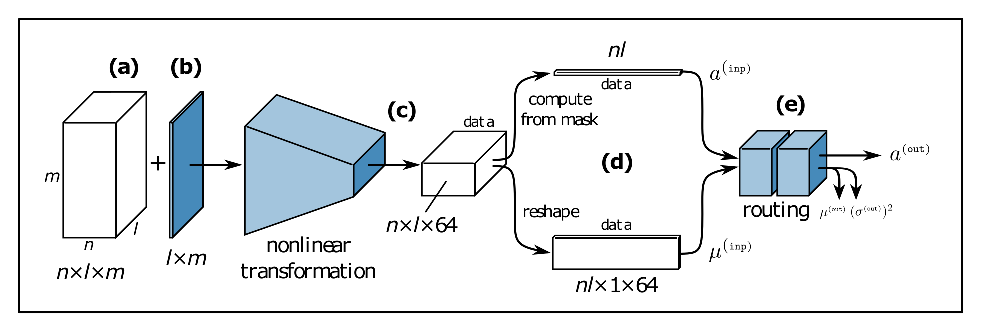
\includegraphics[width=0.9\linewidth]{architecture}
    \caption{Architecture of CapsNet from \cite{heinsen2019algorithm}: (a) For each sample, the input is a tensor of transformer embeddings of
shape $n \times l \times m$, where $n$ is the number of tokens, $l$ is the number of transformer layers, and $m$ is the
embedding size. (b) A depth-of-layer parameter of shape $l \times m$ is element-wise added to the input tensor.
(c) A linear transformation from $m$ to 64 is applied, followed by a Swish activation with constant $\beta = 1$
and layer normalization, obtaining a tensor of shape $n \times l \times 64$. (d) The tensor is reshaped as shown to
obtain $\mu^{(inp)}$, consisting of $ln$ input capsules of size $1\times 64$. The tensor $a^{(inp)} \leftarrow \log \frac{x}{1-x}$ is computed from a mask
$x$ of length $nl$ with ones and zeros indicating, respectively, which embeddings correspond to tokens and
which correspond to any padding necessary to group samples in batches, obtaining logits that are equal
to $\infty$ for tokens, $-\infty$ for padding, and values in between for any tokens and padding that get combined
by mixup regularization in training. (e) Two layers of the routing algorithm are applied; the first one routes
a variable number of capsules in $\mu^{(inp)}$
to 64 capsules of shape $1\times 2$; the second one routes those capsules
to five or two capsules of equal shape, each representing a classification label.
For prediction, we apply a Softmax to output scores $a^{(out)}$.}
    \label{fig:arch}
\end{figure}

\section{Dataset}
GermEval 2017 data was crawled from the Internet on a daily
basis with a list of query terms with the focus on German social media,
microblogs, news, and question and answer sites. From 2.5 million documents spanning a year (May 2015 - June 2016) to capture all possible seasonal problems (holidays, heat, cold, strikes) as well as daily problems such as
delays, canceled trains, or unclear information at the train stations, 1500 documents from each month were sampled for annotation. The annotated data was used for the training,
development, as well as for a {\bf synchronic test set}.
Additionally, to test the robustness of the participating systems, {\bf a diachronic test
set}  was annotated in
the same manner, using data from November 2016
to January 2017.

Totally about 26000 annotated documents for the main dataset were obtained and about 1800 documents for diachronic dataset. The main dataset was split into a training, development and test
set using a random 80\%/10\%/10\% split. Maximal number of tokens in text samples for the training and development dataset is 395, and in the test datasets there is around 1\% of long texts reaching up to 3000 tokens.

The sentiment distribution is presented in Table \ref{tab:sent}. One can observe the huge class disbalance, where the neutral class is a clear majority class. It's notable though that in the diachronic dataset the positive class is much more important so to excel at both tests the solution must deal well with all three classes.  However, due to the absolute prevalence of the neutral class with no useful information, mostly news, the only purpose of this dataset is to test various algorithms on supervised tasks, which were part of GermEval 2017 competition. Other types of analysis such as unsupervised aspect extraction are hard to apply. The ABAE model can correctly identify only one aspect concerning the railway strike which was a hot topic in 2017, and other extracted aspects are completely useless from the point of view of customer analysis and are based solely on the local news around DB, like some politician went to Munich and opened a station. Small part of this dataset could be useful for analysis, however in essence one has to prepare a new dataset and explain what was taken from GermEval 2017 and why.


\begin{table}[tbh!]
\begin{center}
\begin{tabular}[t]{|l|ccc|}
\hline
%\cline{2-4}
Dataset & negative & neutral & positive \\
\hline
Training & 5,045 & 13,208 & 1,179  \\
Development & 589 & 1,632 & 148 \\
Test syn & 780 & 1,681 & 105 \\
Test dia & 497 & 1,237 & 108 \\
\hline
\end{tabular}
\caption{Sentiment Distribution in GermEval 2017.}
\label{tab:sent}
\end{center}
\end{table}


\section{Experiments}
\subsection{Metrics}
The authors of the competition decided to use a F1 micro average metrics, which is equivalent to accuracy when evaluated on all classes:
$$
P = \frac{\sum_i TP_i}{\sum_i TP_i + FP_i}, \quad R = \frac{\sum_i TP_i}{\sum_i TP_i + FN_i}, \quad F1 = \frac{2 P R}{P + R}.
$$
In the situation with a clear majority class this metrics tends to appreciate correct classification into two classes: majority class/other classes, however as mentioned in the previous subsection, since diachronic dataset has different sentiment distribution with more abundant positive class, the algorithm which improves on SOTA for both test datasets has to attend to all the classes.


\subsection{Experiment Setup}
The realization of GPT-2 used in \cite{heinsen2019algorithm} does not support German language, hence we had to replace it with the realization from \\https://github.com/lopuhin/transformer-lm, which realizes GPT-2 architecture with sentencepiece tokenization (50k) and the weights (345 M) for GPT-2$_{medium}$ were downloaded from http://zamia-speech.org/brain/. It does not output hidden layers hence we had to edit the code to use it for our problem. For German BERT we used the FARM framework https://github.com/deepset-ai/FARM similarly to \cite{kostic2020} which operates on top of the standard transformers library \cite{Wolf2019HuggingFacesTS}. We had to integrate CapsNet head into this framework.

First, we trained CapsNet for 5 epochs with batch size 32 and oversampling of positive class by 2 using output of frozen hidden layers of GPT-2 as an input and batch size of 32, learning rate of $10^{-3}$. Maximal length of the tokens in the training dataset is 395 and for evaluation we cut any text at 512 tokens. Other hyperparameters of CapsNet are as in Fig.~\ref{fig:arch}, and the parameters of GPT-2 are $n=1024$, $m=1024$, $l=25$. After that, we unfroze the layers of GPT-2 model, did not do any oversampling, and trained with learning rate of $8\times 10^{-4}$ and batch size 16 for 1 epoch to obtain SOTA results. We note, however, that with the capsule networks due to EM routing it's necessary to perform many runs to end up with the best results \cite{heinsen2019algorithm}. Therefore, we provide the weights to reproduce our SOTA results.

For the BERT backbone ($n=128, l = 14, m=768$) with simple classification head the learning rate was chosen as $3\times 10^{-5}$ for 5 epochs, and for CapsNet head we also trained it with frozen BERT model with the learning rate $10^{-3}$ for 3 epochs, and then unfreeze layers and train for another 3 epochs with learning rate $10^{-4}$. We used batch size of 90 and maximum sequence length 128.


%\subsection{Baselines}
%Another important feature is that you could provide here the description of some simple approaches for your problem, like logistic regression over TF-IDF embedding for text classification. The baselines are needed is there is no previous art on the problem you are presenting.

\section{Results}

We have performed a lot of experiments with both backbone transformer networks, the main results are listed in Table \ref{tab:sent}. We can see that the CapsNet with GPT-2 frozen embeddings improves on the best results of the GermEval 2017 competition, with BERT embeddings it's performing near the current SOTA, with fine-tuned BERT it's as good as the current SOTA, and with fine-tuned GPT-2 it's setting a new SOTA on GermEval 2017 dataset. Nevertheless, we have observed that BERT with CapsNet head consistently underperforms comparing to BERT with simple classification head. The main reason is that the considered architecture (see Fig.~\ref{fig:arch}) is designed to use the power of CapsNets over (fixed) embeddings from the pretrained transformer network. With that it performed well in the original paper using GPT-2$_{large}$ backbone (755 M parameters) \cite{heinsen2019algorithm} and it performs consistently well with GPT-2$_{medium}$ and BERT backbones in this study. However, by fine-tuning BERT after that it was hard to obtain any consistent improvement, the best run gained only 1\% on both test sets, and we never saw any improvements on the typical results of fine-tuned BERT with simple classification head on any of the test sets. 

Remarkably, while CapsNet with frozen GPT-2 embeddings performed a bit worse than CapsNet with BERT embeddings, the end-to-end fine-tuned network with GPT-2 backbone and CapsNet head performed consistently on par with fine-tuned BERT with classification head (current SOTA on GermEval 2017 dataset) and with careful choice of hyperparameters and several runs it's demonstrating the best results on this dataset.  
It's interesting to note that in our experiments increasing maximum sequence length larger than 128 does not improve the performance of BERT classification, however limiting sequence length to 128 in GPT-2 based classification clearly reduces the performance on test datasets, which contain larger texts. It suggests that GPT-2 as a larger network can embed long-range relations that are out of reach of the BERT. 

\begin{table}[tbh!]
\begin{center}	
\begin{tabular}[t]{|l|ccc|}
\hline
%\cline{2-4}
Approach & Synchronic  & Diachronic \\
\hline
Best GermEval2017 \cite{germevaltask2017} & 0.749 & 0.75  \\ % \cite{naderalvojoud2017germeval} % \cite{sayyed2017idst}
LT-ABSA \cite{ruppert2017lt} & 0.767 & 0.744 \\
GPT-2+CapsNets (frozen) & 0.775 & 0.751 \\
ELMo+GloVe+BCN \cite{biesialska2020sentiment} & 0.782 & - \\
BERT+CapsNets (frozen) & 0.779 & 0.782\\
ELMo+TSA \cite{biesialska2020sentiment} & 0.789 & - \\
BERT+CapsNets (unfrozen) & 0.79 & 0.79 \\
BERT (our run) & 0.804 & 0.793 \\
BERT \cite{kostic2020} & 0.801 & 0.802 \\
GPT-2+CapsNets (unfrozen) & 0.812 & 0.803\\
\hline
\end{tabular}
\caption{F1 micro average scores.}
\label{tab:sent}
\end{center}
\end{table}

\section{Conclusion}
In conclusion, we have compared the performance of several networks using embeddings from pretrained transformers on sentiment classification task of GermEval 2017 dataset, and demonsrated new SOTA. We have studied the performance of CapsNets with these backbones and have shown that without fine-tuning they can demonstrate one of the best results, and with fine tuning of GPT-2 backbone network they demonstrate new SOTA on the considered task. We have discussed the importance of long range relations in the texts for the new SOTA. Finally, CapsNets demonstrate big potential in the field of NLP, however their routing procedure leads to less stability in training comparing to the conventional neural networks.
\bibliographystyle{apalike}
\bibliography{report}
\end{document}
